\documentclass[11pt]{beamer}
\usepackage[T1]{fontenc}
\usepackage[activate]{pdfcprot}
\usepackage[ngerman]{babel}
\usepackage[parfill]{parskip}
\usepackage[utf8]{inputenc}
\usepackage{kurier}
\usepackage{amsmath}
\usepackage{amssymb}
\usepackage{xcolor}
\usepackage{epstopdf}
\usepackage{txfonts}
\usepackage{fancyhdr}
\usepackage{graphicx}
\usepackage{prettyref}
\usepackage{hyperref}
\usepackage{eurosym}
\usepackage{setspace}
\usepackage{units}
\usepackage{eso-pic,graphicx}
\usepackage{icomma}

\definecolor{darkblue}{rgb}{0,0,.5}
\hypersetup{pdftex=true, colorlinks=true, breaklinks=false, linkcolor=black, menucolor=black, pagecolor=black, urlcolor=darkblue}



\setlength{\columnsep}{2cm}


\newcommand{\arcsinh}{\mathrm{arcsinh}}
\newcommand{\asinh}{\mathrm{arcsinh}}
\newcommand{\ergebnis}{\textcolor{red}{\mathrm{Ergebnis}}}
\newcommand{\fehlt}{\textcolor{red}{Hier fehlen noch Inhalte.}}
\newcommand{\betanotice}{\textcolor{red}{Diese Aufgaben sind noch nicht in der Übung kontrolliert worden. Es sind lediglich meine Überlegungen und Lösungsansätze zu den Aufgaben. Es können Fehler enthalten sein!!! Das Dokument wird fortwährend aktualisiert und erst wenn das \textcolor{black}{beta} aus dem Dateinamen verschwindet ist es endgültig.}}
\newcommand{\half}{\frac{1}{2}}
\renewcommand{\d}{\, \mathrm d}
\newcommand{\punkte}{\textcolor{white}{xxxxx}}
\newcommand{\p}{\, \partial}
\newcommand{\dd}[1]{\item[#1] \hfill \\}

\renewcommand{\familydefault}{\sfdefault}
\renewcommand\thesection{}
\renewcommand\thesubsection{}
\renewcommand\thesubsubsection{}


\usetheme{Marburg}
\usecolortheme{default}

\useinnertheme{default}
\useoutertheme{default}

\beamertemplatenavigationsymbolsempty
\setbeamertemplate{footline}[frame number]

\title{Galaxien}

\subtitle{Eigenschaften und Klassifikation}

\author{Christoph Hansen}

\institute[FH Aachen - Jülich]{Physikingenieurwesen \\ Fachhochschule Aachen-Jülich}

\date[22.05.14]{22. Mai 2014}

\subject{Eigenschaften und Klassifikation von Galaxien}

\keywords{Galaxien, Eigenschaften, Klassifikation, Hubble}






\begin{document}


%Titelseite

\begin{frame}
\titlepage
\end{frame}


%Inhaltsverzeichnis

\begin{frame}
\tableofcontents
\end{frame}


\section{Überblick über die Klassifikation}

\begin{frame}
\frametitle{Überblick über die Klassifikation}
\framesubtitle{Klassifikation allgemein}

\begin{itemize}
\item Klassifikation hängt von der Beobachtung ab
\end{itemize}
\qquad $\Rightarrow$ Hubbles morphologisches Schema



\begin{itemize}
\item Weitere Möglichkeiten
\begin{enumerate}
\item spektrale Analyse
\item Emissions- und Absorptionsspektrum
\end{enumerate}
\end{itemize}

\end{frame}


\begin{frame}
\frametitle{Überblick über die Klassifikation}
\framesubtitle{Klassifikation nach Hubble}
\begin{figure}
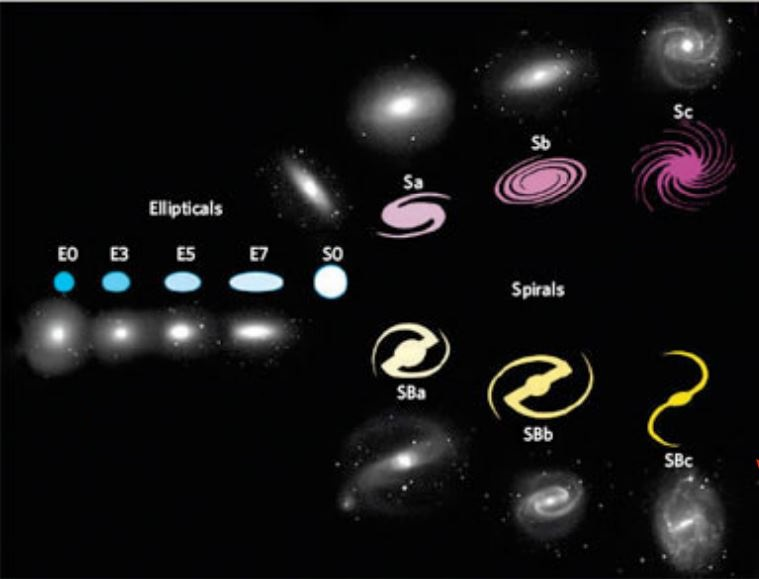
\includegraphics[scale=0.5]{Hubble_Entwicklung.jpg}
\end{figure}
\end{frame}




\begin{frame}
\frametitle{Überblick über die Klassifikation}
\framesubtitle{Klassifikation nach Hubble}

\begin{itemize}
\item keine Entwicklungssequenz
\item zu geringe Anzahl
\item nur optisch
\item zuerst nur drei Typen
\item nutzlos für Leuchtkraft und Entfernungsmessung
\item $\unit[34]{\%}$ Spiralgalaxien, $\unit[13]{\%}$ Ellipsen, $\unit[53]{\%}$ irreguläre Galaxien
\end{itemize}

\end{frame}

\begin{frame}
\frametitle{Überblick über die Klassifikation}
\framesubtitle{Spektralanalyse}

\begin{figure}
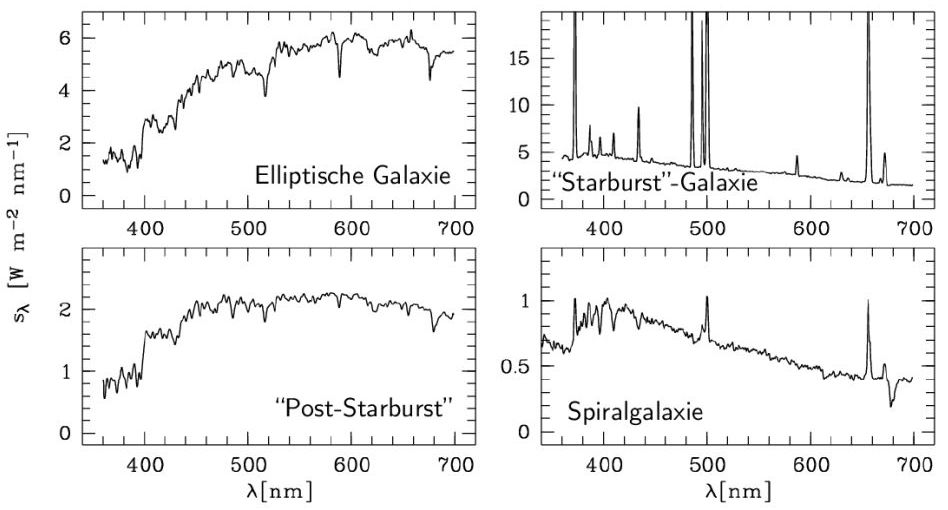
\includegraphics[scale=0.4]{Galaxiespektren.jpg}
\end{figure}

\begin{itemize}
\item Rotverschiebung $z = \frac{\lambda_{beo} - \lambda_0}{\lambda_0}$
\end{itemize}

\end{frame}


\begin{frame}
\frametitle{Überblick über die Klassifikation}
\framesubtitle{Emissions- und Absorbtiosanalyse}


\begin{figure}
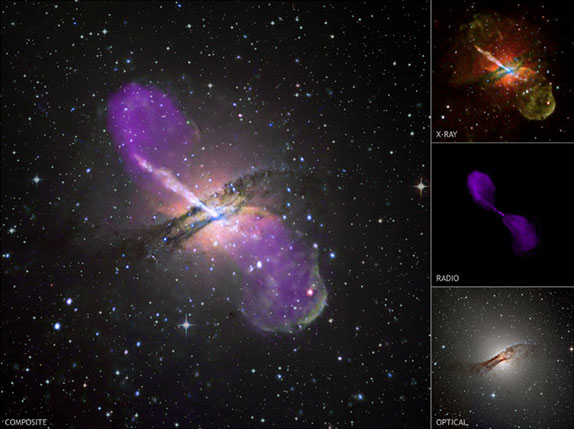
\includegraphics[scale=0.35]{Radiogalaxie.jpg}
\caption{Kombination aus mehreren Wellenlängen}
\end{figure}

\begin{itemize}
\item spezifische Emissionslinien für jeden Typ
\end{itemize}

\end{frame}


\begin{frame}
\frametitle{Überblick über die Klassifikation}
\framesubtitle{Emissions- und Absorbtiosanalyse}

\begin{figure}
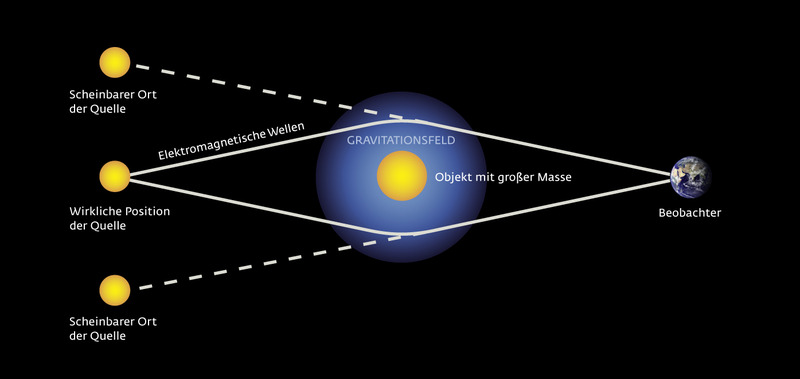
\includegraphics[scale=0.7]{Gravitationslinse.jpg}
\end{figure}

\begin{itemize}
\item indirekter Nachweis
\item Information über Zusammensetzung
\end{itemize}

\end{frame}


\section{Galaxientypen}

\subsection{Elliptische Galaxien}

\begin{frame}
\frametitle{Galaxientypen}
\framesubtitle{Elliptische Galaxien - Namensgebung}



\begin{figure}
\begin{minipage}[hbt]{5cm}
	\centering
	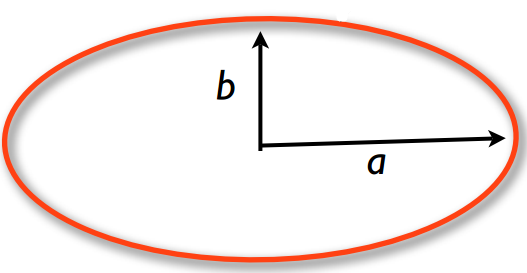
\includegraphics[width=5cm]{Ellipse_Exzentri.png}
	\caption{$\epsilon = 1 - b/a$}
\end{minipage}
\hfill
\begin{minipage}[hbt]{7cm}
	\centering
	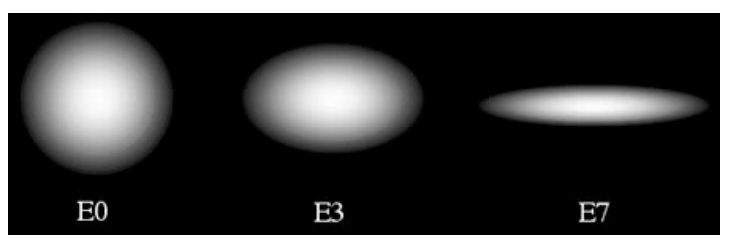
\includegraphics[width=7cm]{Ellipse_Exzentri2.png}
	\caption{$En = E 10\epsilon$}
\end{minipage}
\end{figure}

\end{frame}


\begin{frame}
\frametitle{Galaxientypen}
\framesubtitle{Elliptische Galaxien - Boxyness und Discynes}

%\begin{figure}
%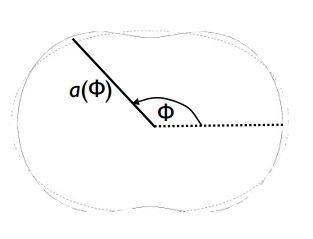
\includegraphics[scale=0.4]{boxi_diski_Schema.jpg}
%\end{figure}

\begin{figure}
\begin{minipage}[hbt]{4cm}
	\centering
	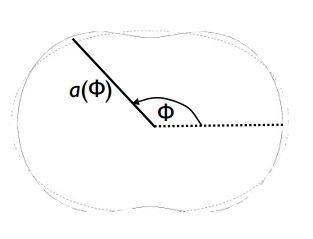
\includegraphics[width=3cm]{boxi_diski_Schema.jpg}
\end{minipage}
%
\begin{minipage}[hbt]{4cm}
	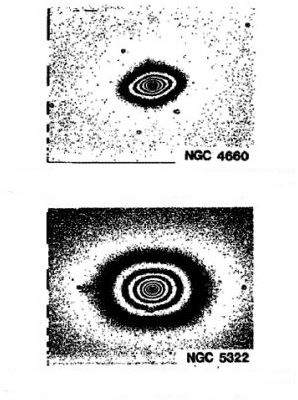
\includegraphics[width=3cm]{boxi_diski_Bild.jpg}
\end{minipage}
\end{figure}


\begin{align*}
a(\phi) &= \underbrace{a_0}_{\text{Kreis}} + \underbrace{a_2}_{\text{Ellipse}} \cos(2 \phi) + \underbrace{a_4}_{\text{Korrektur}} \cos(4 \phi) + \cdots
\end{align*}

\begin{itemize}
\item boxy $\iff$ $a_4/a_0 < 0$ 
\item discy $\iff$ $a_4/a_0 > 0$
\end{itemize}


\end{frame}


\begin{frame}
\frametitle{Galaxientypen}
\framesubtitle{Elliptische Galaxien - verschiedene Klassen}

\begin{figure}
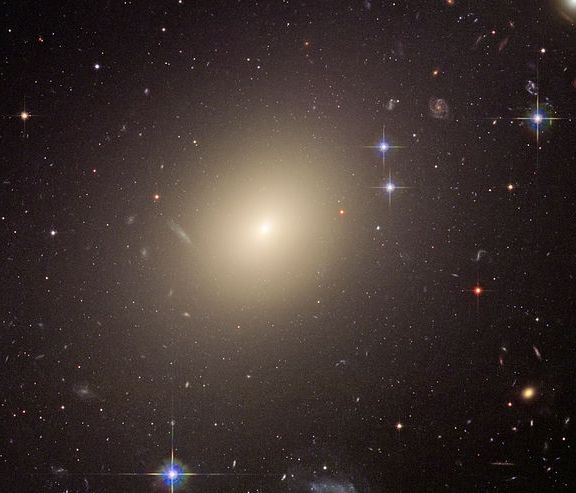
\includegraphics[scale=0.2]{Abell_Ellipise.jpg}
\end{figure}

\begin{itemize}
\item breite Klasse
\item normele Ellipsen haben $\unit[-23]{mag} < M_B < \unit[-15]{mag}$, cD Ellpisen bis $M_B \approx \unit[-15]{mag}$
\end{itemize}

\end{frame}


\begin{frame}
\frametitle{Galaxientypen}
\framesubtitle{Elliptische Galaxien - Helligkeiten}

\hfill \\

\begin{figure}
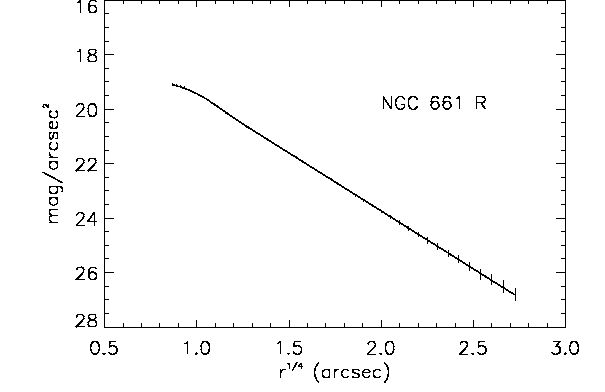
\includegraphics[scale=0.25]{Helligkeitsprofil_Ellipse.jpg}
\end{figure}


\begin{align*}
&\log_{10} \left( \frac{I(R)}{I_e} \right) = - 3,3307 \cdot \left( \sqrt[4]{\frac{R}{R_e}}  - 1 \right) \\
\hfill \\
&L = 2\pi \int_0^\infty R \cdot I(R) \d R = 7,215 \cdot \pi I_e R_e^2
\end{align*}

\end{frame}


\begin{frame}
\frametitle{Galaxientypen}
\framesubtitle{Elliptische Galaxien - Helligkeiten}

\hfill \\

\begin{figure}
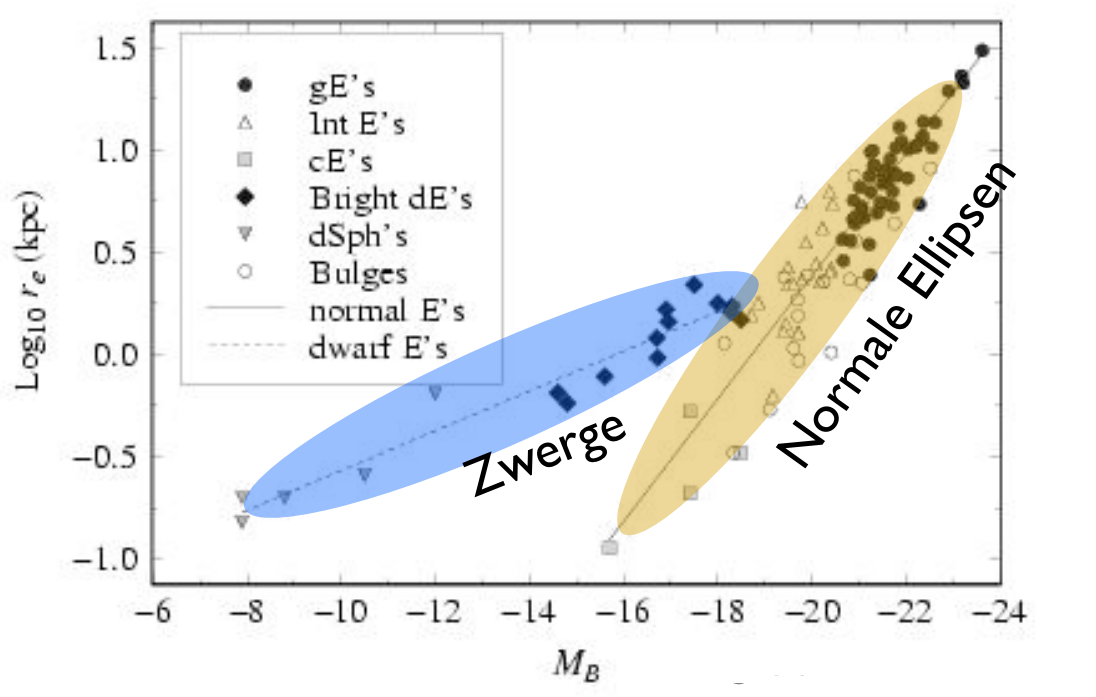
\includegraphics[scale=0.25]{Helligkeitesverteilung_Ellipsen.png}
\caption{Helligkeitsverteilung EG}
\end{figure}



\end{frame}




\begin{frame}
\frametitle{Galaxientypen}
\framesubtitle{Elliptische Galaxien - Zusammensetzung}

\begin{itemize}
\item[1)] heißes Gas $\approx \unit[10^7]{K}$ \\
\item[2)] warmes Gas bei $\approx \unit[10^4]{K}$ $\rightarrow$ $H_\alpha$ Emissionslinien
\item[3)] kaltes Gas mit HI-Linie
\item[4)] Metall - ungleich verteilt
\item[5)] Staub 
\end{itemize}

\end{frame}


\begin{frame}
\frametitle{Galaxientypen}
\framesubtitle{Elliptische Galaxien - Kinematik}

\begin{itemize}
\item Bewegung der Staubscheibe unabhängig vom Rest
\item ungeordnete Bewegung der Sterne
\item Stöße spielen keine Rolle
\end{itemize}


\begin{align*}
&v_{\text{rot}} \approx \sqrt{\frac{\epsilon}{1 - \epsilon}} \cdot \sigma_{\text{v}} \qquad \text{mit} \qquad \epsilon = 1 - c/a
\end{align*}

\end{frame}


\subsection{Spiralgalaxien}

\begin{frame}
\frametitle{Galaxientypen}
\framesubtitle{Spiralgalaxien - Namensgebung}

\begin{figure}
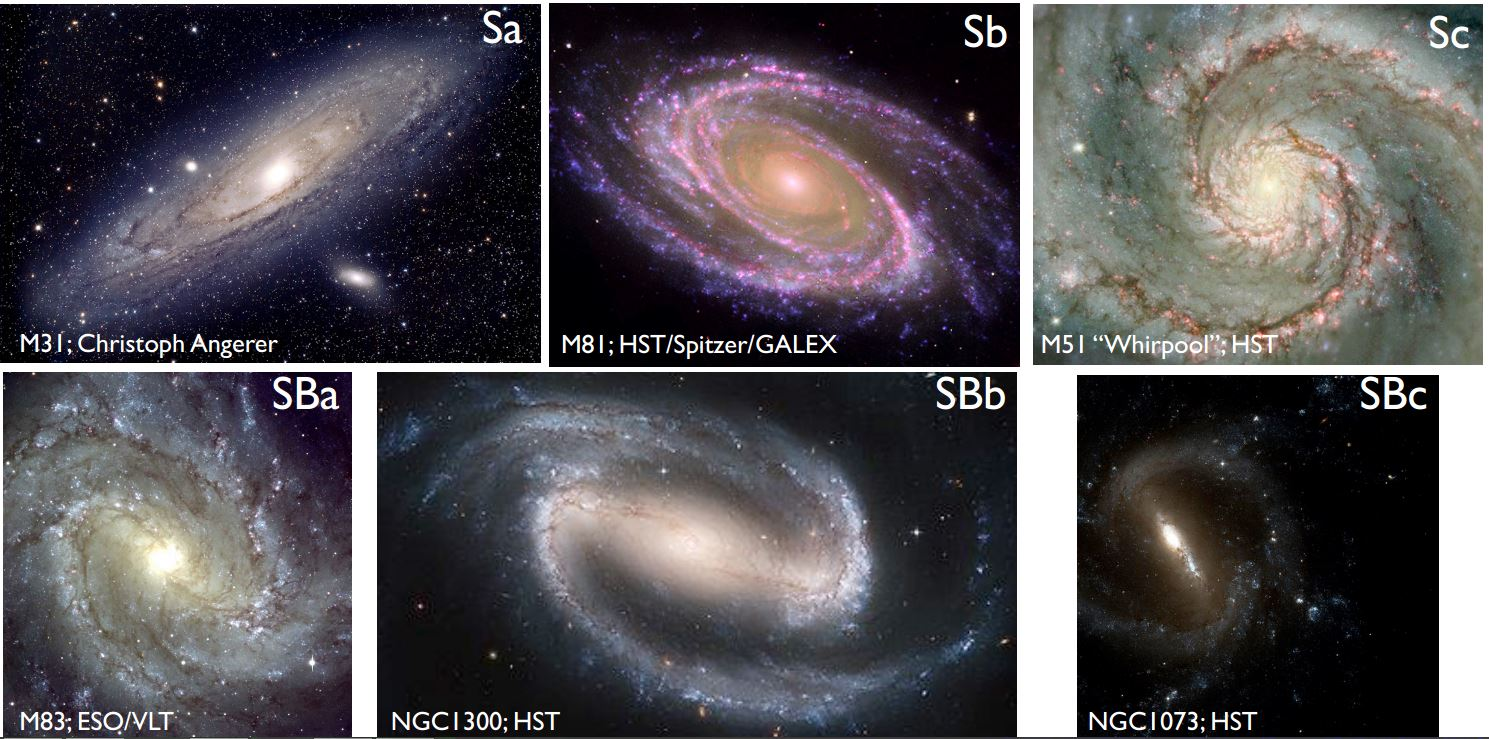
\includegraphics[scale=0.25]{Spiral_Namensgebung.jpg}
\end{figure}

\begin{itemize}
\item Gasgehalt
\item Verhältnis Bulge/Scheibe
\item Öffnungswinkel
\end{itemize}

\end{frame}


\begin{frame}
\frametitle{Galaxientypen}
\framesubtitle{Spiralgalaxien - Helligkeitsprofil}

\begin{figure}
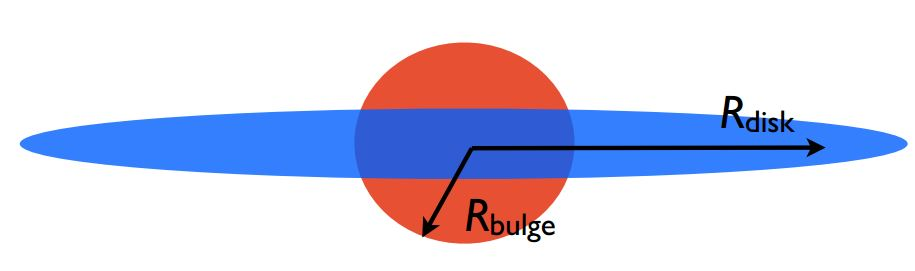
\includegraphics[scale=0.25]{Spiralgalaxie_Schema.jpg}
\end{figure}

\begin{align*}
&\mu \left( R_{\text{Bulge}} \right) = \mu_e + 8,3268 \cdot \left( \sqrt[4]{\frac{R_{\text{Bulge}}}{R_e}} - 1 \right) \\
\hfill \\
\hfill \\
&\mu \left( R_{\text{Disc}} \right) = \mu_0 \cdot e^{-\frac{r}{r_0}}
\end{align*}

\end{frame}


\begin{frame}
\frametitle{Galaxientypen}
\framesubtitle{Spiralgalaxien - Rotation}

\begin{figure}[h]
	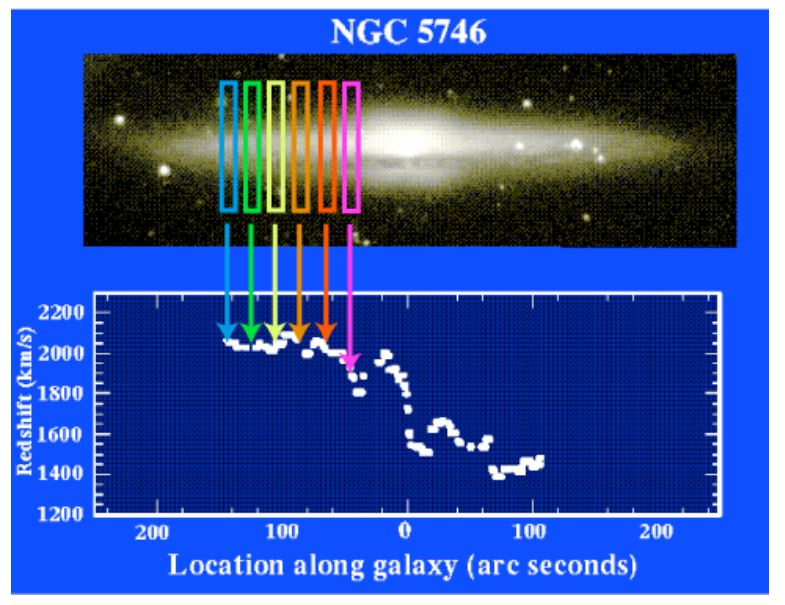
\includegraphics[scale=0.4]{Spiralgalaxie_Rotation1.jpg}
	\caption{Rotaionsgeschwindigkeiten bei SG}
\end{figure}

\end{frame}




\begin{frame}
\frametitle{Galaxientypen}
\framesubtitle{Spiralgalaxien - Rotation}


\begin{figure}
	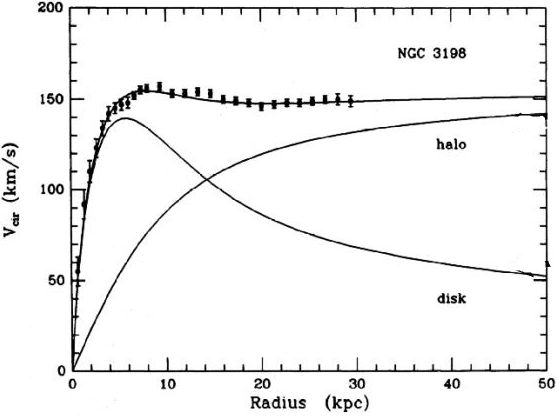
\includegraphics[scale=0.35]{Spiralgalaxie_Rotation2.jpg}
\end{figure}

\begin{itemize}
\item Rotationskurven nicht durch sichtbare Materie erklärbar
\end{itemize}


\begin{align*}
M_{\text{dark}} = \frac{r}{G} \left( v^2(r) - v_{\text{lum}}^2(r) \right)
\end{align*}

\end{frame}




\begin{frame}
\frametitle{Galaxientypen}
\framesubtitle{Spiralgalaxien - Sternentstehung}

\begin{figure}
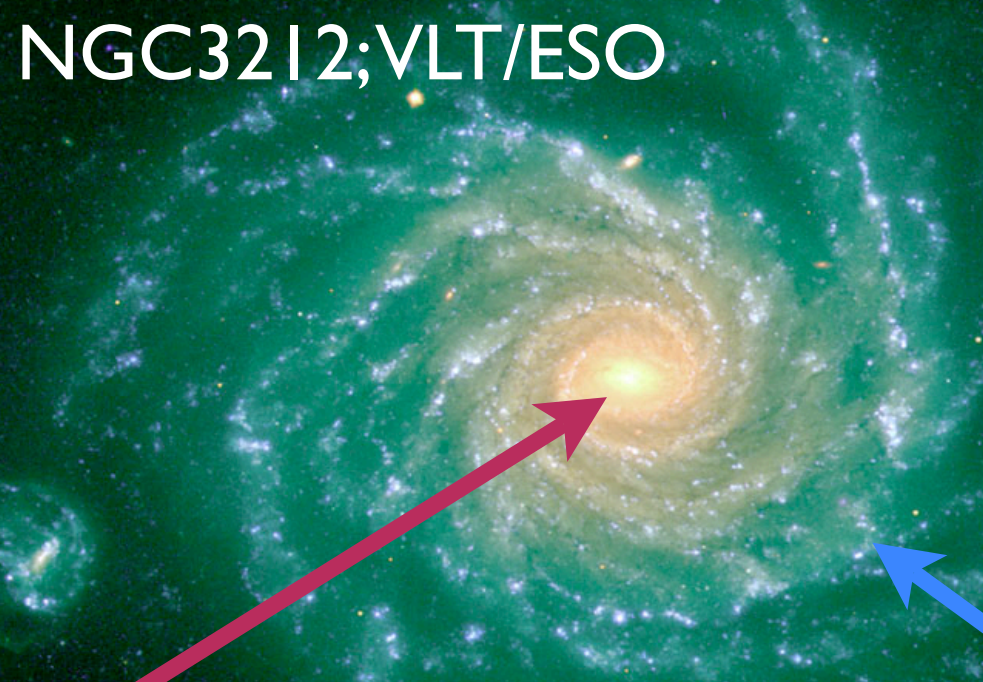
\includegraphics[scale=0.25]{Sternentstehung_Spirale.png}
\end{figure}

\begin{itemize}
\item je jünger, desto mehr Sterne
\item findet in den Armen statt
\end{itemize}

\end{frame}


\begin{frame}
\frametitle{Galaxientypen}
\framesubtitle{Spiralgalaxien - Spiralstruktur}


\begin{itemize}
\item quasi stationäre Dichtewellen 
\item Kompression im Arm
\item Sterne bleiben lebenslang in den Armen
\end{itemize}

\end{frame}


\begin{frame}
\frametitle{Quellen}
\framesubtitle{ }


\begin{itemize}
\item Die Welt der Galaxien - Prof. Peter Schneider \& Dr. Patrick Simon
\item Einführung in die Astronomie II - Peter Schneider
\item Eigenschaften normaler Galaxien - unbekannt
\item Einführung in die Astronomie \& Astrophysik II - Wilhelm Kley
\end{itemize}

\end{frame}



\end{document}